\begin{center}
	\LARGE
	Uden hjælpemidler
\end{center}
\begin{opgavetekst}{Opgave 1}
	To mængder $A$ og $B$ er givet ved
	\begin{align*}
		A &= \{1,2,3,4,5\}, \\
		B &= \{2,4,5,6,a,b\}.
	\end{align*}
\end{opgavetekst}
\begin{delopgave}{}{1}
	Bestem $A \cup B$, $A \cap B$ og $A \backslash B$. 
\end{delopgave}
\begin{delopgave}{}{2}
	For to vilkårlige mængder $S$ og $T$ tegn da et Venn-diagram, der illustrerer mængden 
	\begin{align*}
		(S\cup T)\backslash (S\cap T)
	\end{align*}
\end{delopgave}
\begin{delopgave}{}{3}
	Bestem mængden $C$ givet ved
	\begin{align*}
		C = (A\cup B)\backslash (A \cap B).
	\end{align*}
\end{delopgave}
\begin{opgavetekst}{Opgave 2}
	En funktion $f$ er givet ved grafen på Figur \ref{fig:defværd}
	\begin{figure}[H]	
	\centering
	\resizebox{0.45\textwidth}{!}{
	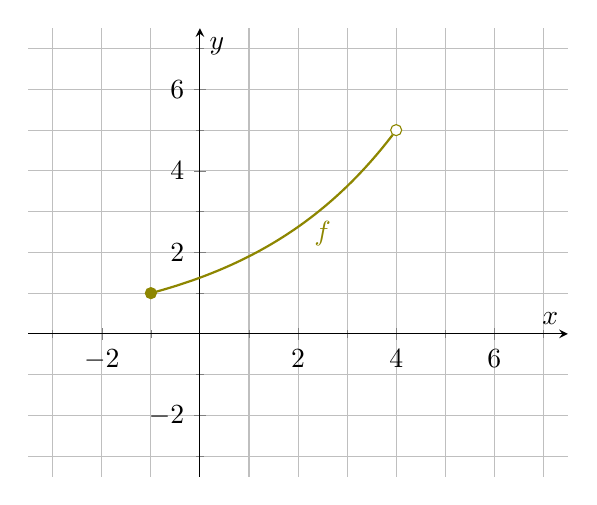
\begin{tikzpicture}
		\begin{axis}
		[axis lines = center, 
		xmin = -3.5, xmax = 7.5,
		ymin = -3.5, ymax = 7.5,
		grid = both,
		xtick = {-4,-2,...,8,10},
		ytick = {-4,-2,...,8,10},
		minor tick num = 1,
		xlabel = $x$, ylabel = $y$
		]
			\addplot[color = olive, thick, domain = -1:4, samples = 200] {1.3797*1.3797^x};	
			\filldraw[color = white](axis cs: 4,5) circle (2pt);
			\draw[color = olive](axis cs: 4,5) circle (2pt);
			\filldraw[color = olive](axis cs: -1,1) circle (2pt);
			\node[color = olive, anchor = north] at (axis cs: 2.5,3) {$f$};
		\end{axis}
	\end{tikzpicture}
	}
	\caption{Graf for funktionen $f$.}
	\label{fig:defværd}
	\end{figure}
	\phantom{h}
\end{opgavetekst}
\begin{delopgave}{}{1}
	Bestem $f(-1)$.
\end{delopgave}
\begin{delopgave}{}{2}
	Bestem definitionsmængden $\textnormal{Dm}(f)$ og værdimængden $\textnormal{Vm}(f)$.
\end{delopgave}

\newpage

\begin{opgavetekst}{Opgave 3}
	En funktion $f: \mathbb{R} \to \mathbb{R}$ er givet ved
	\begin{align*}
		f(x) = 4x-5.
	\end{align*}	 
\end{opgavetekst}

\begin{delopgave}{}{1}
	For mængden $A = \{1,3,5\}$ bestem da billedmængden $f(A)$.
\end{delopgave}
\begin{delopgave}{}{2}
	Bestem urbilledet af $B = \{-9,20,-5\}$ under $f$.
\end{delopgave}

\begin{opgavetekst}{Opgave 4}
	To funktioner $f$ og $g$ er givet ved henholdsvis
	\begin{align*}
		f(x) &= \log_{2}(x), \\
		g(x) &= x^2 - 4x + 4 
	\end{align*}
\end{opgavetekst}
\begin{delopgave}{}{1}
	Bestem $f(g(6))$.
\end{delopgave}

\newpage

\begin{opgavetekst}{Opgave 5}
	Grafen for en stykvist defineret funktion $g$ kan ses af Figur \ref{fig:stykvis}.
	\begin{figure}[H]
		\centering
		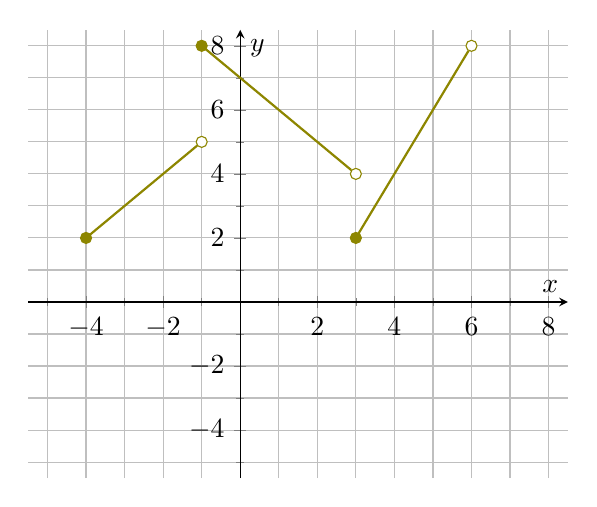
\begin{tikzpicture}
		\begin{axis}
		[
		axis lines = middle, 
		xmin = -5.5, xmax = 8.5,
		ymin = -5.5, ymax = 8.5,
		xtick = {-6,-4,...,8,10},
		ytick = {-6,-4,...,8,10},
		minor tick num = 1,
		xlabel = $x$, ylabel = $y$,	
		grid = both,	
		]
			\addplot[color = olive, thick, domain = -4:-1] {x + 6};
			\addplot[color = olive, thick, domain = -1:3] {-x + 7};
			\addplot[color = olive, thick, domain = 3:6] {2*x - 4};
			\filldraw[color = olive] (axis cs: -4,2) circle (2pt);
			\filldraw[color = white] (axis cs: -1,5) circle (2pt);
			\draw[color = olive] (axis cs: -1,5) circle (2pt);
			\filldraw[color = olive] (axis cs: -1,8) circle (2pt);
			\filldraw[color = white] (axis cs: 3,4) circle (2pt);
			\draw[color = olive] (axis cs: 3,4) circle (2pt);
			\filldraw[color = olive] (axis cs: 3,2) circle (2pt);
			\filldraw[color = white] (axis cs: 6,8) circle (2pt);
			\draw[color = olive] (axis cs: 6,8) circle (2pt);
		\end{axis}
		\end{tikzpicture}
		\caption{Graf for funktionen $g$.}
		\label{fig:stykvis}
	\end{figure}
	\phantom{h}
\end{opgavetekst}
\begin{delopgave}{}{1}
	Opskriv en forskrift for funktionen $g$.
\end{delopgave}
\begin{delopgave}{}{2}
	Bestem løsningerne til ligningen $g(x) = 4$.
\end{delopgave}

\newpage 

\begin{opgavetekst}{Opgave 6}
	Grafen for en funktion $h:[-4,3[ \to [-4,5]$ er givet på Figur \ref{fig:injsur}.
	\begin{figure}[H]
		\centering
		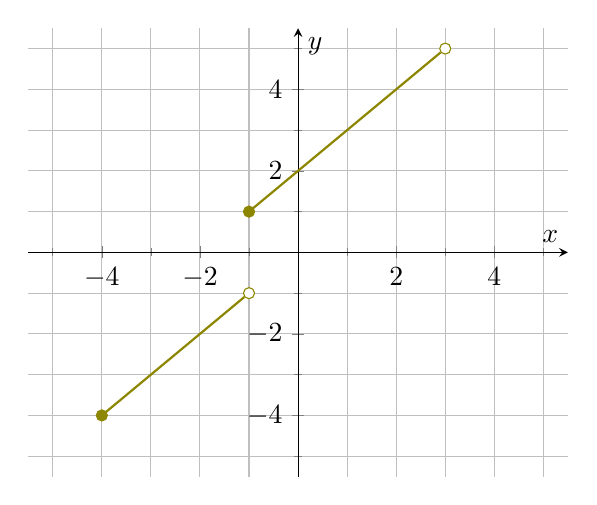
\begin{tikzpicture}
		\begin{axis}
		[
		axis lines = middle, 
		xmin = -5.5, xmax = 5.5,
		ymin = -5.5, ymax = 5.5,
		xtick = {-6,-4,...,8,10},
		ytick = {-6,-4,...,8,10},
		minor tick num = 1,
		xlabel = $x$, ylabel = $y$,	
		grid = both,	
		]
			\addplot[color = olive, thick, domain = -4:-1] {x};
			\addplot[color = olive, thick, domain = -1:3] {x + 2};
			\filldraw[color = olive] (axis cs: -4,-4) circle (2pt);
			\filldraw[color = white] (axis cs: -1,-1) circle (2pt);
			\draw[color = olive] (axis cs: -1,-1) circle (2pt);
			\filldraw[color = olive] (axis cs: -1,1) circle (2pt);
			\filldraw[color = white] (axis cs: 3,5) circle (2pt);
			\draw[color = olive] (axis cs: 3,5) circle (2pt);
		\end{axis}
		\end{tikzpicture}
		\caption{Graf for funktionen $h$.}
		\label{fig:injsur}
	\end{figure}
	\phantom{h}
\end{opgavetekst}
\begin{delopgave}{}{1}
	Afgør, om $h$ er surjektiv, injektiv eller bijektiv. Begrund dit svar.
\end{delopgave}

\begin{opgavetekst}{Opgave 7}
	To funktioner $f$ og $g$ er givet ved henholdsvis
	\begin{align*}
		f(x) &= 5^{3x-7}, \\
		g(x) &= \frac{\log_{5}(x) + 7}{3}.
	\end{align*}
\end{opgavetekst}
\begin{delopgave}{}{1}
	Undersøg, om $f$ og $g$ er hinandens inverse funktioner.
\end{delopgave}	
\begin{delopgave}{}{2}
	Bestem den inverse funktion til $f$ givet ved
	\begin{align*}
		f(x) = 10x - 6.
	\end{align*}
\end{delopgave}

